\section{FSA-v5: Adding Sedentary Collapse to Match Medical Reality} \label{sec:fsa-v5-sketch}

The FSA-v4 model has a structural feature that sits awkwardly with exercise medicine: the autonomic amplitude $A$ does \emph{not} collapse under chronic inactivity. Setting $\Phi = 0$ (full sedentary) gives the model a low-but-nonzero attractor $A^* \approx 0.32$ rather than $A = 0$. Empirically, prolonged sedentary inactivity does impair autonomic regulation --- reduced heart-rate variability, blunted baroreflex sensitivity, and in extreme deconditioning, autonomic dysfunction. This section presents the minimal extension of FSA-v4 --- ``FSA-v5'' --- that closes the gap, simulates it qualitatively, and explains how to calibrate the new parameters from a single subject's longitudinal data (the N=1 setting this codebase is being prepared for).

\subsection{Why FSA-v4 misses sedentary collapse}

Setting $\Phi = (0, 0)$ in the closed-form equilibria of Section \ref{sec:fsa-v4-stability} gives $B^* = S^* = F^* = 0$, and hence
\begin{equation}
\bar\mu_{\rm v4}(0;\, 0) \;=\; \mu_0 - \mu_{FF} F_{\rm TYP}^2 \;=\; 0.036 - 0.4 \cdot 0.04 \;=\; +0.020 \;>\; 0.
\label{eq:v4-mu0-sedentary}
\end{equation}
Strictly positive, so the boundary equilibrium $A = 0$ at zero training is locally unstable: the system rises to a small interior $A^* > 0$. The healthy basin survives all the way down to $\Phi = 0$. Pictorially, the v4 transcritical curve $\bar\mu(0;\Phi) = 0$ is an open quarter-disc in $(\Phi_B, \Phi_S)$-space (left panel of Figure \ref{fig:v5_island}). For the model to fit medical reality the topology must change: the healthy region needs to be a \emph{closed} subset of stimulus space, with collapsed regimes on \emph{both} sides --- low $\Phi$ (deconditioning) and high $\Phi$ (over-training).

\subsection{The minimal mathematically principled fix: Hill-function deconditioning}

The cleanest modification preserves every piece of the FSA-v4 cascade structure (Section \ref{sec:v4-cascade}) and adds a single \emph{smooth} non-linear deconditioning term to the bifurcation parameter:
\begin{equation}
\bar\mu_{\rm v5}(A;\Phi) \;=\; \bar\mu_{\rm v4}(A;\Phi) \;-\; \mu_{B-} \cdot \frac{B_{\rm dec}^{n}}{B^*(A)^{n} + B_{\rm dec}^{n}} \;-\; \mu_{S-} \cdot \frac{S_{\rm dec}^{n}}{S^*(A)^{n} + S_{\rm dec}^{n}}.
\label{eq:v5-mubar}
\end{equation}
Each Hill term is a saturating dose--response curve in the chronic-fitness state:
\begin{itemize}
  \item At full deconditioning ($B \to 0$): the term saturates at $\mu_{B-}$ (max penalty applied).
  \item At the threshold ($B = B_{\rm dec}$): the term equals $\mu_{B-}/2$.
  \item At well-trained states ($B \gg B_{\rm dec}$): the term falls to zero (no penalty).
\end{itemize}
The Hill exponent $n$ controls the steepness of the transition; we use $n = 4$ as a default, giving a smooth-but-sharp sigmoidal cut-off. This is the natural functional form for a saturating physiological dose--response and is $C^\infty$ everywhere (no kinks), so it integrates cleanly with both gradient-based and SMC-based inference.

\paragraph{Why this is principled, not a hack.}
\begin{enumerate}
  \item \textbf{The cascade structure is unchanged.} The $K$, $(B,S)$, $F$ blocks are untouched; equations (\ref{eq:K-star})--(\ref{eq:F-star}) of Section \ref{sec:fsa-v4-stability} carry through unmodified. The slow-manifold equilibria, the block-triangular Jacobian, and the composite Lyapunov function are all preserved verbatim. \emph{All} that changes is the location of the bifurcation curves in stimulus space and the size of $\bar\mu$.
  \item \textbf{Detraining-timescale physics emerges naturally.} A previously-trained athlete who turns sedentary has $B(t), S(t)$ relaxing on their intrinsic time-scales $\tau_B = 42$ d, $\tau_S = 60$ d. The Hill term grows smoothly as $B$ drops below $B_{\rm dec}$. So $\bar\mu$ stays positive while the athlete remains conditioned, then crosses zero, and only then does $A$ collapse. The model predicts the empirically-observed weeks-to-months detraining time-course of autonomic decline (see the simulation in Section \ref{sec:v5-trajectories} below).
  \item \textbf{Four scalar parameters per modality, all with direct medical interpretation.} $B_{\rm dec}, S_{\rm dec}$ are the chronic-fitness thresholds below which autonomic dysfunction emerges. $\mu_{B-}, \mu_{S-}$ are the maximum autonomic-drive reductions in the fully deconditioned state. $n$ is the steepness of the transition. All dimensionless or in the same units as the existing model.
  \item \textbf{Self-consistency reduces to the same scalar equation.} The interior equilibria of $A$ still solve $\bar\mu(A;\Phi) = \eta A^2$, just with $\bar\mu_{\rm v5}$ in place of $\bar\mu_{\rm v4}$. The transcritical surface is still $\bar\mu(0;\Phi) = 0$, the saddle-node still where the two roots collide. Every analytical and numerical tool of Section \ref{sec:fsa-v4-stability} re-runs verbatim --- only the drift function in \texttt{models/fsa\_high\_res/\_dynamics.py} needed editing, and only by adding the two Hill subtractions.
\end{enumerate}

\subsection{Closed-island basin topology --- both modalities required}

Figure \ref{fig:v5_island} shows the transcritical bifurcation contour $\bar\mu(0;\Phi) = 0$ for v4 (left) versus v5 (right) using the parameter values $B_{\rm dec} = S_{\rm dec} = 0.07$, $\mu_{B-} = \mu_{S-} = 0.10$, $n = 4$. The healthy region collapses from an open quarter-disc to a closed island whose interior is strictly bounded away from both coordinate axes. This is medically essential: the boundary $\Phi_B = 0$ corresponds to ``no aerobic training'' and the boundary $\Phi_S = 0$ to ``no strength training''. A model that admits a healthy attractor on either axis would be predicting that strength-only or aerobic-only training is sufficient for autonomic resilience --- empirically incorrect. The new parameters were scanned to produce an island whose boundary is strictly interior to $(\Phi_B, \Phi_S) \in \mathbb{R}_{>0}^2$, encoding the requirement that \emph{both} aerobic and strength stimuli are necessary for sustained autonomic health.

\begin{table}[h]
\centering
\small
\begin{tabular}{lcl}
\toprule
Stimulus regime & $\bar\mu(0;\Phi)$ & Outcome \\
\midrule
Sedentary, $\Phi = (0, 0)$               & $-0.180$ & strong collapse \\
Aerobic-only, $\Phi = (0.30, 0)$         & $-0.059$ & collapse \\
Strength-only, $\Phi = (0, 0.30)$        & $-0.093$ & collapse \\
Balanced moderate, $\Phi = (0.30, 0.30)$ & $+0.011$ & \textbf{healthy} ($A^* \approx 0.54$) \\
Over-training, $\Phi = (1.0, 1.0)$       & $-1.608$ & catastrophic collapse \\
\bottomrule
\end{tabular}
\caption{Numerical confirmation of the FSA-v5 closed-island topology with the scanned parameter set $B_{\rm dec} = S_{\rm dec} = 0.07$, $\mu_{B-} = \mu_{S-} = 0.10$, $n = 4$. Only balanced bilateral training places the system inside the healthy island; \emph{both} axes (aerobic-only or strength-only) lie outside it.}
\label{tab:v5_island_check}
\end{table}

Outside the island in any direction --- sedentary, aerobic-only, strength-only, over-training, or any combination --- $\bar\mu(0;\Phi) < 0$ and $A = 0$ is locally stable. Table \ref{tab:v5_island_check} reports the values at five representative points; only the balanced-moderate configuration gives a positive $\bar\mu$ and a healthy interior attractor.

\begin{figure}[h]
    \centering
    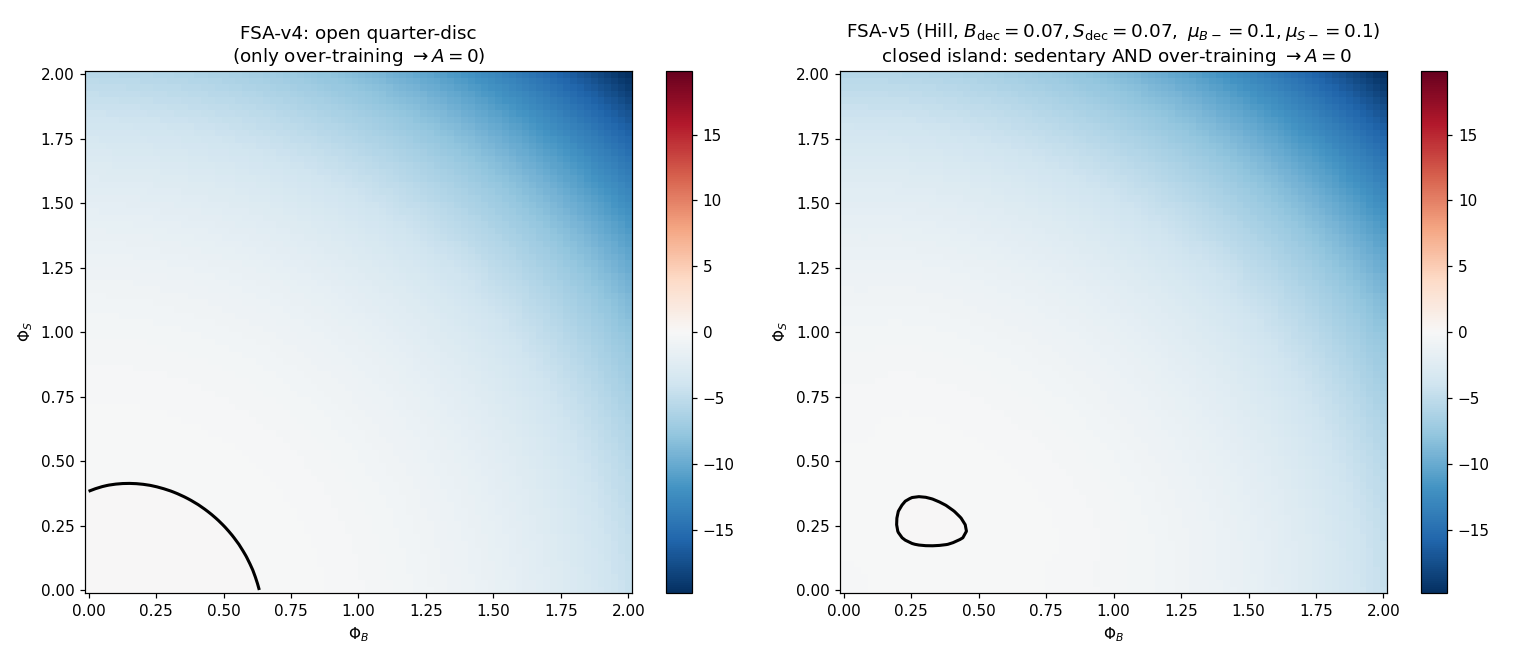
\includegraphics[width=\textwidth]{figures/v5_sedentary_collapse_island.png}
    \caption{Comparison of the transcritical bifurcation contour under FSA-v4 (left) and FSA-v5 (right). v4 admits a healthy regime down to $\Phi = 0$ \emph{and} along the $\Phi_S = 0$ axis (i.e.\ aerobic-only training would suffice). The v5 Hill-deconditioning term ($B_{\rm dec} = S_{\rm dec} = 0.07,\ \mu_{B-} = \mu_{S-} = 0.10,\ n=4$) closes the contour into a closed island whose boundary is strictly interior to both coordinate axes. The medical ``Goldilocks'' / inverse-U structure emerges as a basin-topology change, encoding the requirement that both aerobic and strength stimuli are necessary for autonomic health.}
    \label{fig:v5_island}
\end{figure}

The full three-region structure of Section \ref{sec:fsa-v4-stability} carries over to the closed island. Figure \ref{fig:v5_full_bifurcation} adds the saddle-node curve (magenta dashed): inside the black transcritical island the regime is mono-stable healthy; in the annulus between black and magenta it is bistable; outside the magenta it is mono-stable collapsed. The right panel confirms the analytical structure with a numerical sweep of forward rollouts from $A_0 = 0.05$.

\begin{figure}[h]
    \centering
    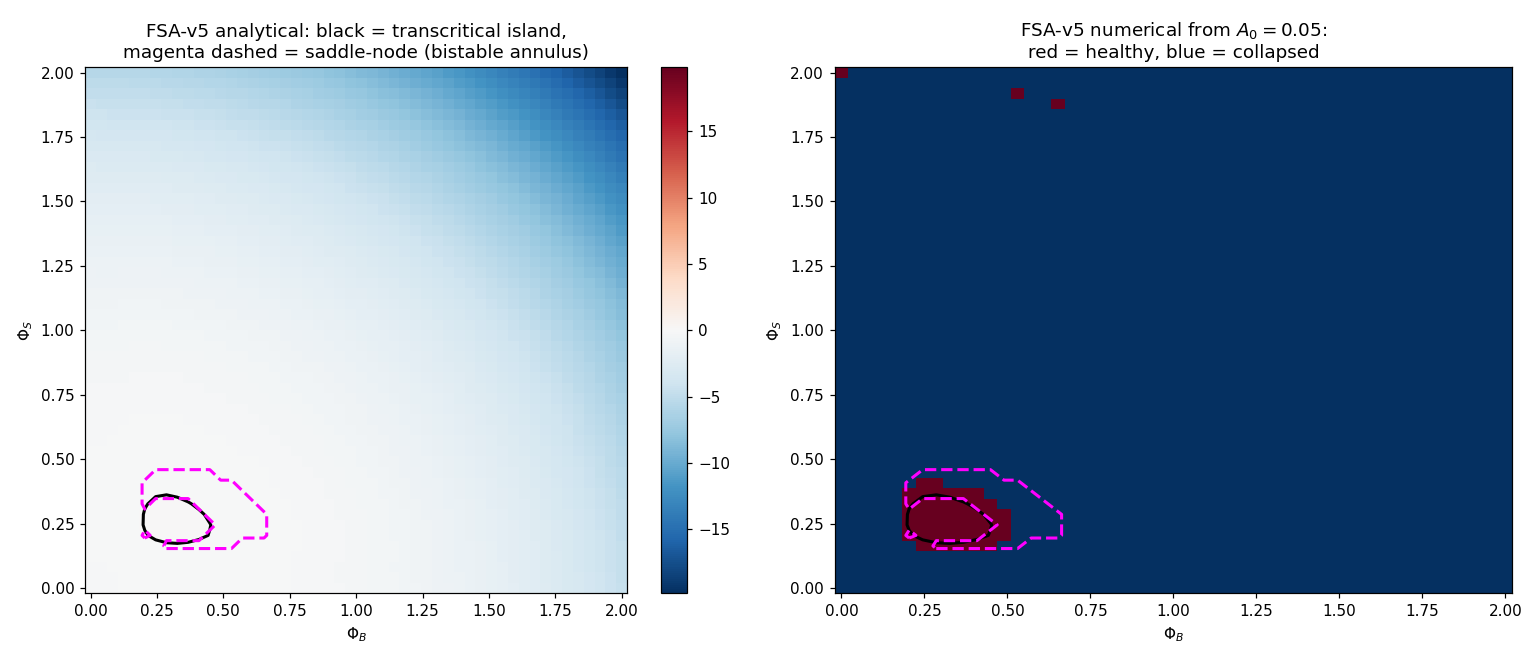
\includegraphics[width=\textwidth]{figures/v5_full_bifurcation.png}
    \caption{FSA-v5 full bifurcation diagram. Left: analytical transcritical (black) and saddle-node (magenta dashed) contours on the heatmap of $\bar\mu(0;\Phi)$. Right: numerical regime classification from forward RK4 rollouts with $A_0 = 0.05$. The bistable annulus surrounds the healthy island on all sides --- both deconditioning and over-training are reachable from a small initial $A$.}
    \label{fig:v5_full_bifurcation}
\end{figure}

\subsection{Equilibrium values across the stimulus plane} \label{sec:v5-eq-table}

Table \ref{tab:v5_equilibrium_values} reports the closed-form equilibrium properties at a $6\times 6$ grid in $(\Phi_B, \Phi_S)$. The pattern is striking and confirms the closed-island topology numerically:

\begin{itemize}
  \item All sedentary rows ($\Phi_B \le 0.15$): collapsed. $\bar\mu(0;\Phi) < 0$, no positive interior root.
  \item All over-training rows ($\Phi_B \ge 0.70$): collapsed. The v4 F-mediated mechanism dominates.
  \item The middle band ($\Phi_B \in \{0.30, 0.45\}$ at moderate $\Phi_S$): healthy or bistable. Only at $\Phi_B = 0.30$, $\Phi_S \in \{0.15, 0.30\}$ is the regime mono-stable healthy --- a tiny island at moderate, balanced training.
\end{itemize}

\begin{table}[h]
    \centering
    \scriptsize
    \begin{tabular}{cc|ccccc}
\toprule
$\Phi_B$ & $\Phi_S$ & $\bar\mu(0;\Phi)$ & $A^*$ (stable) & $A_{\rm sep}$ & $B^*$ & Regime \\
\midrule
0.05 & 0.05 & $-0.169$ & --- & --- & 0.025 & collapsed \\
0.05 & 0.15 & $-0.118$ & --- & --- & 0.025 & collapsed \\
0.05 & 0.30 & $-0.086$ & --- & --- & 0.025 & collapsed \\
0.05 & 0.45 & $-0.112$ & --- & --- & 0.025 & collapsed \\
0.05 & 0.70 & $-0.235$ & --- & --- & 0.025 & collapsed \\
0.05 & 1.00 & $-0.590$ & --- & --- & 0.025 & collapsed \\
0.15 & 0.05 & $-0.103$ & --- & --- & 0.076 & collapsed \\
0.15 & 0.15 & $-0.053$ & --- & --- & 0.076 & collapsed \\
0.15 & 0.30 & $-0.025$ & --- & --- & 0.076 & collapsed \\
0.15 & 0.45 & $-0.054$ & --- & --- & 0.076 & collapsed \\
0.15 & 0.70 & $-0.185$ & --- & --- & 0.076 & collapsed \\
0.15 & 1.00 & $-0.555$ & --- & --- & 0.076 & collapsed \\
0.30 & 0.05 & $-0.058$ & --- & --- & 0.151 & collapsed \\
0.30 & 0.15 & $-0.011$ & --- & --- & 0.151 & collapsed \\
0.30 & 0.30 & $+0.011$ & $0.543$ & --- & 0.184 & healthy \\
0.30 & 0.45 & $-0.027$ & $0.439$ & $0.180$ & 0.178 & bistable \\
0.30 & 0.70 & $-0.178$ & --- & --- & 0.151 & collapsed \\
0.30 & 1.00 & $-0.578$ & --- & --- & 0.151 & collapsed \\
0.45 & 0.05 & $-0.062$ & --- & --- & 0.227 & collapsed \\
0.45 & 0.15 & $-0.020$ & $0.322$ & $0.212$ & 0.256 & bistable \\
0.45 & 0.30 & $-0.007$ & $0.600$ & $0.033$ & 0.281 & bistable \\
0.45 & 0.45 & $-0.057$ & --- & --- & 0.227 & collapsed \\
0.45 & 0.70 & $-0.235$ & --- & --- & 0.227 & collapsed \\
0.45 & 1.00 & $-0.680$ & --- & --- & 0.227 & collapsed \\
0.70 & 0.05 & $-0.133$ & --- & --- & 0.353 & collapsed \\
0.70 & 0.15 & $-0.101$ & --- & --- & 0.353 & collapsed \\
0.70 & 0.30 & $-0.110$ & --- & --- & 0.353 & collapsed \\
0.70 & 0.45 & $-0.189$ & --- & --- & 0.353 & collapsed \\
0.70 & 0.70 & $-0.430$ & --- & --- & 0.353 & collapsed \\
0.70 & 1.00 & $-0.976$ & --- & --- & 0.353 & collapsed \\
1.00 & 0.05 & $-0.392$ & --- & --- & 0.504 & collapsed \\
1.00 & 0.15 & $-0.378$ & --- & --- & 0.504 & collapsed \\
1.00 & 0.30 & $-0.422$ & --- & --- & 0.504 & collapsed \\
1.00 & 0.45 & $-0.549$ & --- & --- & 0.504 & collapsed \\
1.00 & 0.70 & $-0.895$ & --- & --- & 0.504 & collapsed \\
1.00 & 1.00 & $-1.608$ & --- & --- & 0.504 & collapsed \\
\bottomrule
\end{tabular}
    \caption{FSA-v5 equilibrium values. $\bar\mu(0;\Phi)$ is the linearisation of $A$ at the boundary equilibrium; sign determines stability of $A=0$. $A^*$ is the largest positive root of $g(A) = \bar\mu(A;\Phi) - \eta A^2 = 0$ (stable interior); $A_{\rm sep}$ is the smaller root (unstable separatrix). $B^*$ is the slow-manifold aerobic-fitness equilibrium at the corresponding $A$.}
    \label{tab:v5_equilibrium_values}
\end{table}

\subsection{Time-domain simulation: both tails drive collapse} \label{sec:v5-trajectories}

The static tables only show steady states. To verify the dynamics actually \emph{traverse} from a healthy initial state to $A=0$ under sedentary or over-training input --- on physiologically reasonable timescales --- we run the full deterministic 6D ODE under three constant-$\Phi$ scenarios from a common ``trained athlete'' initial state $(B_0, S_0, F_0, A_0, K_{FB,0}, K_{FS,0}) = (0.50, 0.45, 0.20, 0.45, K_{FB}^*(0.5), K_{FS}^*(0.5))$.

\begin{figure}[h]
    \centering
    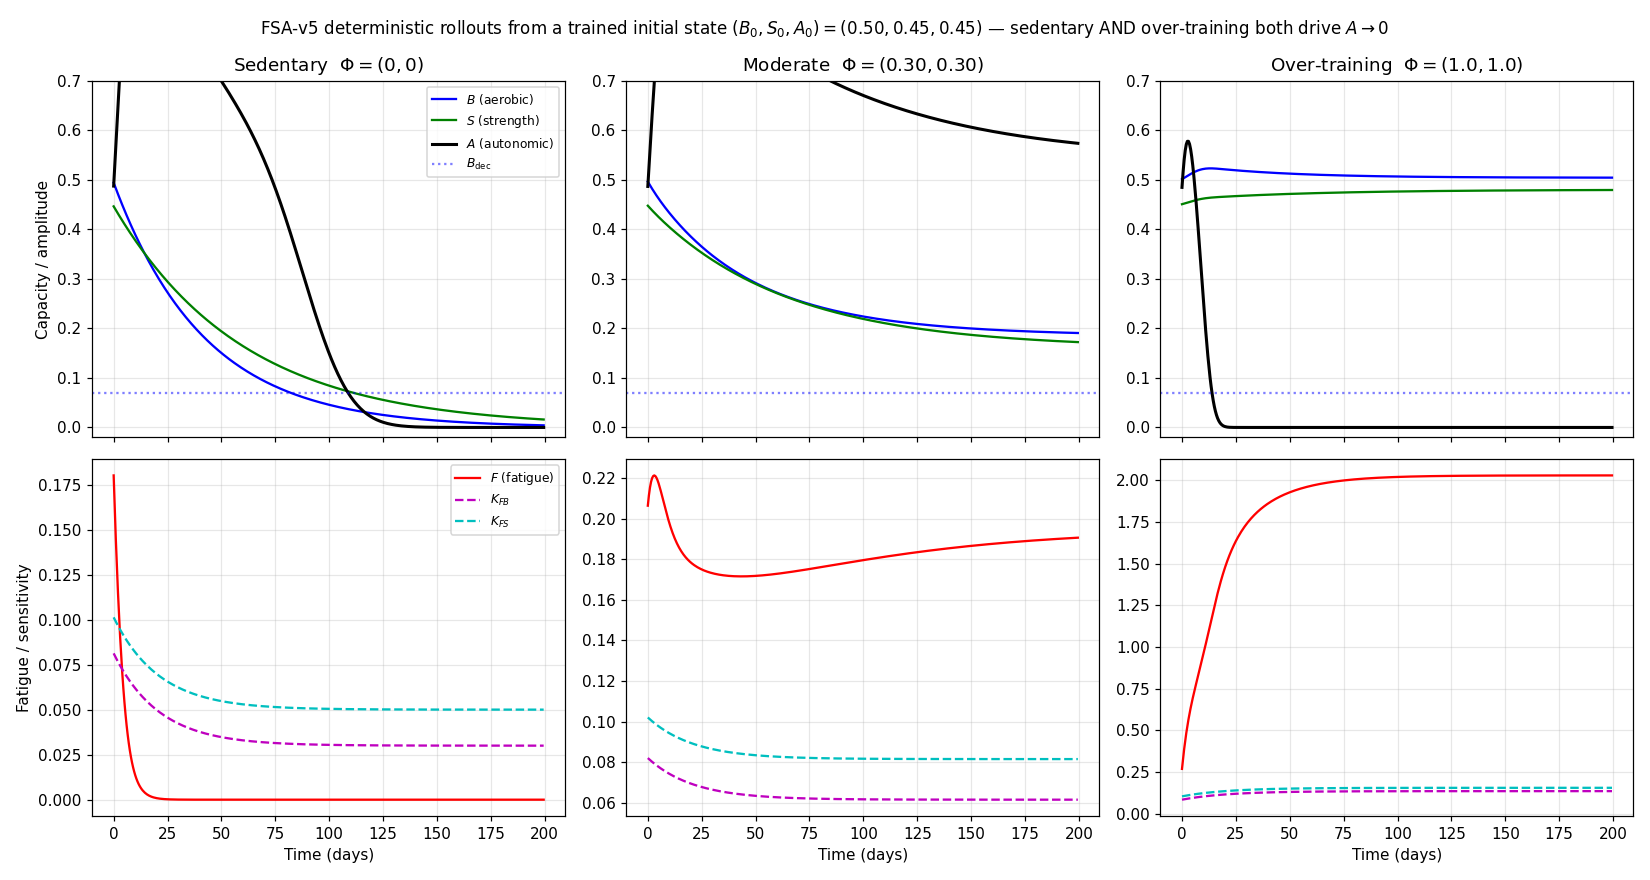
\includegraphics[width=\textwidth]{figures/v5_trajectories_three_regimes.png}
    \caption{FSA-v5 deterministic RK4 rollouts from a trained initial state, under three constant-$\Phi$ regimes. Top row: chronic-fitness states $B$ (blue), $S$ (green), and autonomic amplitude $A$ (black). Bottom row: fatigue $F$ (red) and dynamic fatigue gains $K_{FB}, K_{FS}$. Both sedentary ($\Phi=0$) and over-training ($\Phi=(1,1)$) drive $A \to 0$, but via different physiological mechanisms (deconditioning of $B,S$ vs.\ runaway $F$). Only the moderate scenario ($\Phi=(0.3,0.3)$, inside the v5 island) maintains $A$ at a healthy value.}
    \label{fig:v5_trajectories}
\end{figure}

The qualitative behaviour visible in Figure \ref{fig:v5_trajectories} is exactly what was sought:

\paragraph{Sedentary ($\Phi=0$).} $B$ and $S$ decay exponentially at their intrinsic rates ($\tau_B = 42$ d, $\tau_S = 60$ d). Around day 40--60, both fall below the deconditioning threshold $B_{\rm dec} = S_{\rm dec} = 0.07$ (dashed reference line in the top-left panel) and the Hill terms in (\ref{eq:v5-mubar}) saturate. With $\bar\mu$ now strongly negative ($\bar\mu(0;0) = -0.18$, see Table \ref{tab:v5_island_check}), $A$ collapses to zero by day 120. Fatigue $F$ also decays (no input), and $K$ relaxes to baseline. \emph{Sedentary collapse is mediated by detraining of the chronic capacities, not by fatigue.}

\paragraph{Moderate balanced ($\Phi=(0.3, 0.3)$, inside the v5 island).} Both modalities are non-zero, $B$ and $S$ both clear the deconditioning threshold $B_{\rm dec} = S_{\rm dec} = 0.07$, and the Hill terms remain near zero. $\bar\mu(0; (0.3, 0.3)) = +0.011$ stays positive; the interior attractor sits at $A^* \approx 0.54$ (Table \ref{tab:v5_island_check}). $A$ relaxes to that value over $\sim$100 days. Fatigue $F$ stabilises near $F_{\rm TYP} = 0.20$, $K$ rises modestly to its slow-manifold values. \emph{Goldilocks-band homeostasis} --- and crucially this only works because \emph{both} $\Phi_B$ and $\Phi_S$ are non-zero; the same total stimulus delivered as aerobic-only or strength-only would land outside the island.

\paragraph{Over-training ($\Phi=(1,1)$).} $B$ saturates at 0.5, $S$ rises sharply, but fatigue $F$ runs away to $\approx 2$ (10$\times$ above $F_{\rm TYP}$) within 30 days. The v4 fatigue-mediated mechanism dominates: $\bar\mu$ goes strongly negative because of the $-\mu_{FF}(F-F_{\rm TYP})^2$ term, and $A$ collapses to zero by day $\sim$50. Note that this collapse is much \emph{faster} than the sedentary one --- minutes-to-days rather than weeks-to-months --- because the F-runaway is driven by an active stimulus, whereas detraining is passive decay. \emph{Over-training collapse is mediated by fatigue, not deconditioning.}

This dual-mechanism picture is medically reasonable. Acute over-training crashes happen on a much shorter time-scale than slow deconditioning autonomic loss, and they manifest differently (high $F$ at collapse vs.\ low $F$ at collapse). The same model now captures both.

\subsection{Calibration for N=1 longitudinal study}

This codebase is being prepared for inference against a single subject's own time-series data. The user (Ajay) has reasonable subjective annotations of which periods of his own history correspond to detraining, balanced training, and over-training, plus longitudinal HRV / resting heart rate / sleep / VO$_2$max-proxy measurements over those periods. In this setting the right calibration strategy is a \emph{parameter scan} for qualitative-realistic behaviour, not a fit against published cohort data:

\begin{enumerate}
  \item \textbf{Why not cohort calibration.} Population-level studies of HRV vs. cardiorespiratory fitness show high inter-individual variance and meaningful but modest correlation; for example, see Marco Altini's discussion of the literature. Pinning the FSA-v5 deconditioning thresholds against a population mean would import that variance into the N=1 model and likely give less individual realism than tuning to the subject's own observed transitions.
  \item \textbf{What to scan.} The four new parameters $B_{\rm dec}, S_{\rm dec}, \mu_{B-}, \mu_{S-}$ (with $n$ fixed at 4 unless visibly mismatched). For each candidate combination:
    \begin{itemize}
      \item Simulate the v5 trajectory under the subject's actual logged $\Phi(t)$ schedule across known annotated periods (e.g., a 6-week detraining episode followed by 6 weeks of moderate training).
      \item Compare the predicted $A(t)$ against the observed HRV proxy (or a smoothed version of it).
      \item Accept parameter combinations that produce qualitatively correct timing of autonomic decline / recovery --- not point-by-point exact fits, but the right time-scale and the right ordering of events.
    \end{itemize}
  \item \textbf{Identifiability.} The four v5 parameters are identifiable in this N=1 setting only if the subject's logged history spans both tails: at least one prolonged taper / detraining episode (informs $\mu_{B-}, \mu_{S-}$) and at least one episode of sustained high load (informs the v4 $\mu_F, \mu_{FF}$ already, but also bounds the upper extent of the island). Annotated personal history is uniquely well-suited for this.
  \item \textbf{Soft anchors from physiology.} $B_{\rm dec}$ should sit near the value of $B$ that the subject reaches after $\sim 3$ weeks of complete inactivity (roughly 1--2 weeks past the typical short-illness window). $\mu_{B-}$ should be large enough that sedentary $\bar\mu(0;0)$ is clearly negative (visible HRV decline within $\sim$2 months) but small enough that the healthy island is not microscopic.
  \item \textbf{Uncertainty.} The SMC$^2$ inference framework of Section \ref{sec:smc2_vs_ot} naturally maintains a posterior over the four v5 parameters --- so the user does not need to commit to point values. Each parameter particle simulates a v5 trajectory and is re-weighted against observation likelihood. This is the right framework for the under-constrained N=1 problem.
\end{enumerate}

\subsection{Implications for downstream control}

The cost-function design of Section \ref{sec:fsa-v4-cost} carries over without change: the recommended objective is still $-\int A\, dt + \lambda_\Phi \int \|\Phi\|^2 + \lambda_K \int \|K - K^0\|^2$, plus optional $B,S$ targeting for concurrent goals. Under v5, the chance constraint $\Pr[A_t < A_{\rm sep}(\Phi_t)] \le \alpha$ now excludes a band on the \emph{low-$\Phi$} side as well as the high. The SMC$^2$ controller (Section \ref{sec:smc2_vs_ot}) handles both walls equally well; it simply rejects $\theta$-particles that simulate trajectories crossing into either the deconditioning or the over-training collapsed basin at the prescribed rate.

\subsection{Steps for porting v5 into the \texttt{smc2fc} repository}

The v5 modification is a strict super-set of v4: setting $\mu_{B-} = \mu_{S-} = 0$ recovers v4 dynamics exactly. So the port can proceed in two stages:

\begin{enumerate}
  \item Import \texttt{models/fsa\_high\_res/\_dynamics.py} (with the Hill term already integrated into \texttt{drift\_jax}) and \texttt{TRUTH\_PARAMS\_V5} into \texttt{smc2fc}. With $\mu_{B-} = \mu_{S-} = 0$, all existing v4 behaviour is preserved.
  \item Add $B_{\rm dec}, S_{\rm dec}, \mu_{B-}, \mu_{S-}$ to the SMC$^2$ parameter vector $\theta$, with informative priors centred on the scan-determined values from the N=1 calibration above.
\end{enumerate}

The stability tool \texttt{tools/stability\_basins\_v4.py} already handles both v4 and v5 by accepting the truth-params dictionary as an argument; it can be ported directly as a verification utility.
